\documentclass[czech,bachelor]{diploma}

\usepackage[autostyle=true,czech=quotes]{csquotes} % korektni sazba uvozovek, podpora pro balik biblatex
\usepackage[backend=biber, style=iso-numeric, alldates=iso]{biblatex} % bibliografie
\usepackage{dcolumn} % sloupce tabulky s ciselnymi hodnotami
\usepackage{subfig} % makra pro "podobrazky" a "podtabulky"

\usepackage{float} % lepsi umistovani obrazku (H)

% Pozadovane vstupy pro generovani titulnich stran.
\ThesisAuthor{Barbora Kovalská}
\ThesisSupervisor{doc. Ing. Radoslav Fasuga, Ph.D.}

\CzechThesisTitle{Tvorba herního modelu výpravné evoluční hry}
\EnglishThesisTitle{Creation of the Game Model for the Narrative Evolution Game}

\SubmissionYear{2024}

\ThesisAssignmentFileName{../specification.pdf}

\Acknowledgement{Ráda bych nepoděkovala svému minulému já za to, že se rozhodla na práci nepracovat.}

\CzechAbstract{Tato bakalářská práce se zabírá vytvořením a dokumentací herního systému pro hybridní deskovou hru.}
\CzechKeywords{desková hra; herní design}

\EnglishAbstract{This bachelor's thesis deals with the creation and documentation of a game system for a hybrid board game.}
\EnglishKeywords{board game; game design}

\AddAcronym{TTS}{Trails Through Shadows}
\AddAcronym{RPG}{Role Playing Game}

\addbibresource{Resources/websites.bib}

% Novy druh tabulkoveho sloupce, ve kterem jsou cisla zarovnana podle desetinne carky
\newcolumntype{d}[1]{D{,}{,}{#1}}


% Zacatek dokumentu
\begin{document}

% Titulni strany
\MakeTitlePages

% Seznam obrazku
\listoffigures
\clearpage

% Seznam tabulek
\listoftables
\clearpage

% Text zaverecne prace.
\chapter{Úvod}

Welcome to hell. This is the introduction chapter.

\chapter{Teorie a analýza}
\label{ch:theory_and_analysis}
V této kapitole se budeme věnovat teorii a analýze rozhraní, včetně jejich klíčových prvků, které jsou zásadní pro pochopení základních principů efektivního designu jak uživatelských (UI), tak i administrativních rozhraní. Dále se zaměříme na analýzu populárních deskových her, které si v současné době získaly velkou popularitu a zájem hráčů. V závěru této kapitoly se zaměříme na administrativní prvky a značky, které jsou zásadní pro správu obsahu aplikace.

\section{Teorie UI/GUI}
\label{sec:ui-gui-theory}
Uživatelské rozhraní z anglického jazyka \textit{\textquote{User Interface}} (UI) a grafické uživatelské rozhraní \textit{\textquote{Graphical User Interface}} (GUI) jsou termíny používány v kontextu digitálních aplikací, kde tyto komponenty umožňují uživatelům interagovat se softwárem aplikace pomocí rozhraní. Zatímco UI zahrnuje jakoukoliv formu uživatelského rozhraní, GUI se specificky zaměřuje na vizuální aspekty rozhraní jako jsou okna, ikony, tlačítka a další grafické elementy.

Základem dobrého UI je především jeho intuitivita, jednoduchost a přehlednost, což jednoduše znamená, že by uživatel měl být schopen jednoduše pochopit jak s aplikačním rozhraním pracovat, aniž by musel procházet složitějším procesem učení.

\subsection*{Klíčové prvky UI/GUI}
\label{subsec:ui-gui-theory-key-elements}
\begin{itemize}
    \item \textbf{Rozložení} -- Efektivní rozložení usnadňuje uživatelskou orientací, uživatelé pak snadnější naleznou potřebné funkce nebo informace.
    \item \textbf{Prvky ovládání} -- Tlačítka, menu, přepínače a další administrativní prvky by měly být v ideálním případě jasně označené a snadno dostupné.
    \item \textbf{Typografie a barevnost} -- Výběr písma a jeho barevné schéma hraje významnou roli v čitelnosti a celkovém vnímání. V dnešní době se stránky hodně zaměřují na tmavá přepínatelná pozadí často známá jako \textit{Dark Mode} a \textit{Light Mode}.
    \item \textbf{Interaktivita} -- Při podání vstupu do aplikace by uživatelé měli dostat okamžitou zpětnou vazbu, čímž tak dostávají informace, že jejich akce byla zpracována nebo se aktuálně zpracovává. Často je tak probíhající akce vyobrazena určitým opakujícími se animacemi například tak točící se kolečko známé jako \textit{loading spinner}.
    \item \textbf{Přizpůsobivost} -- Možnost přizpůsobit si uživatelské rozhraní tak zvyšuje celkovou přívětivost, v rozhraních tak většinou nalezneme možnost změnit jazyk, barvy nebo pozice jednotlivých oken. Tyto změny se tak většinou uchovávají pouze v uložišti prohlížeče a nejsou nijak sdílený mezi zařízeními.
\end{itemize}

\subsection*{Principy dobrého UI designu}
\label{subsec:ui-gui-theore-basic-use-case}
\begin{itemize}
    \item \textbf{Konzistence} -- Při provádění stejné akce, by uživatel měl pokaždé dostat stejnou odpověď.
    \item \textbf{Jednoduchost} -- UI by mělo mít minimalistický design, který je hlavně zaměřen na důležité funkce.
    \item \textbf{Přívětivost} -- Uživatel by měl být schopen, okamžitě pochopit rozložení UI bez nutnosti se ho učit.
    \item \textbf{Dostupnost} -- UI by mělo být dostupné pro všechny uživatele, bez ohledu na jejich schopnosti.
    \item \textbf{Zabezpečení} -- UI by mělo být zabezpečené a chránit uživatele před různými útoky.
\end{itemize}

\subsection{Počátek vzniku rozhraní}
\label{subsec:ui-gui-theory-beginning}
Vznik rozhraní lze vysledovat až k raným počátkům počítačů, kde se interakce mezi uživatelem a rozhraním prováděla pomocí děrných štítků a přepínačů. Postupem času s vývojem technologií vzniklo rozhraní terminálové z anglického jazyka \textit{\textquote{Command Line Interface}} (CLI), které obsahovalo základní textový vstup z klávesnice a následného výstupu umístěného na displej. Toto rozhraní se tak stalo standardem pro každý novodobý počítač a používá se do dnešních let. Zlomovým momentem se poté stal příchod grafické rozhraní z angl. \textit{\textquote{Graphical User Interface}} (GUI), které znamenalo revoluci v přístupu k interakci uživatele s počítačem. Tato evoluce přinesla nové možnosti pro uživatele jak přímo komunikovat s počítačem díky grafickým prvkům jako jsou okna, ikony, menu za pomocí pohybu myši po obrazovce.

Pro nás se grafická reprezentace v počítači stala již nedílnou součástí našeho života a v dnešní době se sní setkáváme již na každém kroku, ať se jedná o mobilní aplikace, počítačové aplikace nebo prosté webové stránky.

Pro vývoj webových aplikací se většinou používají technologie spojené pomocí jazyku JavaScript. V minulých letech, zde ale existoval software se jménem \textit{Adobe Flash Player}, který umožňoval vytvářet interaktivní multimediální obsah, které se mnohdy využíval na vývoj různých webových aplikace ať se jednalo o různé hry, prezentace nebo třeba aplikaci fotogalerie. Bohužel tento software byl koncem roku 2020 ukončen a nahrazen modernějšími a bezpečnějšími technologiemi, které zároveň stály za jeho úpadkem. Mezi tyto technologie se tak řadí HTML5, WebGL nebo WebAssembly. \cite{adobeFlashPlayer-eol}

\subsection{Problematika vývoje}
\label{subsec:ui-gui-theory-problems}
Problematika vývoje rozhraní se týká komplexního procesu, který zahrnuje několik oblastí, nad kterými je potřeba se předem zamyslet a následně je implementovat. Většinou při zanedbaní správné implementace těchto sekcí, lze v budoucnu rychle dosáhnout problémům, kde jejich řešení může mít výrazný vliv na funkčnost aplikace. Mezi tyto oblasti spadá například:

\begin{itemize}
    \item \textbf{Uživatelský vstup}, který reprezentuje jakým způsobem bude uživatel nebo administrátor aplikaci podávat vstup. Tedy jestli se jedná o textový vstup, vstup ovládáním myši nebo dotykovým displejem. Dle tohoto kritéria se poté volí vhodný způsob zpracování vstupu.
    \item \textbf{Vykreslování}, které se většinou rozděluje na potřeby uživatelské a administrativní částí. Kde uživatelská se zaměřuje více na design a přívětivost pro uživatele, zatímco administrativní se zaměřuje na efektivitu a snadnou správu obsahu. Tento rozdíl můžeme jednoduše vidět na tom, že administrativní rozhraní často využívá plný potenciál obrazovky, zatímco uživatelské se snaží dbát na přehlednost a jednoduchost.
    \item \textbf{Responzivní design} určuje, jak se jednotlivé prvky v obrazovce zachovají při změně velikosti okna nebo zařízení. Aplikace by v ideálním případě po změně velikosti neměla ztratit na přehlednosti nebo jakkoliv poškodit uživatelskou zkušenost. U mobilních verzí aplikací se tak často objevují separátní odkazy na nativní rozhraní, které se tak často nachází pod subdoménou s název \("\)m\("\) tedy například \textit{https://m.tts-game.fun}. Řešení responzivního designu dále bude pokračovat v separátním odstavci~\ref{subsec:ui-gui-theory-responsive-design}.
    \item \textbf{Uživatelská zkušenost} z anglického jazyka \textit{\textquote{User Experience}} (UX) se soustředí na to, jak uživatelé vnímají a jak se cítí při používání aplikace. Tedy jak je aplikace přívětivá, snadno ovladatelná a zda splňuje očekávání uživatele.
    \item \textbf{Bezpečnost} je důležitým aspektem, který se zaobírá zpracováním uživatelských dat, které v mnoha případech obsahuje citlivé informace. Při nesprávném zpracování těchto dat může dojít k úniku dat nebo zneužití. Jako řešení se používají různé techniky, jako je například šifrování, ověřování uživatele nebo zabezpečení připojení.
\end{itemize}

\subsection{Responzivní design}
\label{subsec:ui-gui-theory-responsive-design}
Responzivní design se stal již skoro povinným standardem pro všechny webové stránky a aplikace. Tento přístup se zaměřuje na webové prvky tak, aby při jejich zobrazení na různých zařízeních s rozdílnou velikosti obrazovky nebo orientace byly pořád stejně přehledné a plně funkční. Této funkčnosti se dosahuje pomocí CSS stylů, které tuto funkcionalitu umožňují pomocí tzv. \textit{\textquote{media queries}}. Tyto dotazy umožňují nastavovat styly podle předem daných kritérii, jako jsou například šířka okna, výška okna, typ zařízení nebo jeho orientace.

Jedním z průkopníků responzivního designu se stal \textit{Bootstrap}, open-source framework pro vývoj front-end webových aplikací. Který nabízí soubor knihoven a předem vytvořených šablon stylů, díky kterým je možné za použití pár elementů dosáhnout rychlého a plně responzivního designu aplikace. Tento framework je v současné době jedním z nejpoužívanějších z důvodu jeho lehkého nasazení, široké podpory a velké kompatibility. Využití potenciálu tohoto frameworku si blíže popíšeme v kapitole~\ref{subsec:dev-technology-bootstrap}.

\lstinputlisting[language=CSS, caption={Příklad použití media query v css.}, label={lst:media-query-example}]{sourceCodes/MediaQueryExample.css}

V stručném vysvětlení kódu~\ref{lst:media-query-example} můžeme vidět, že se jedná o základní CSS kód, který nastavuje barvu pozadí stránky na světle šedou. Ale obsahuje media dotaz na řádku 6, které se ptá na velikost obrazovky, kde v případě, že je šířka obrazovka menší než 600px, změní barvu pozadí na světle modrou.

\begin{figure}[H]
    \centering
    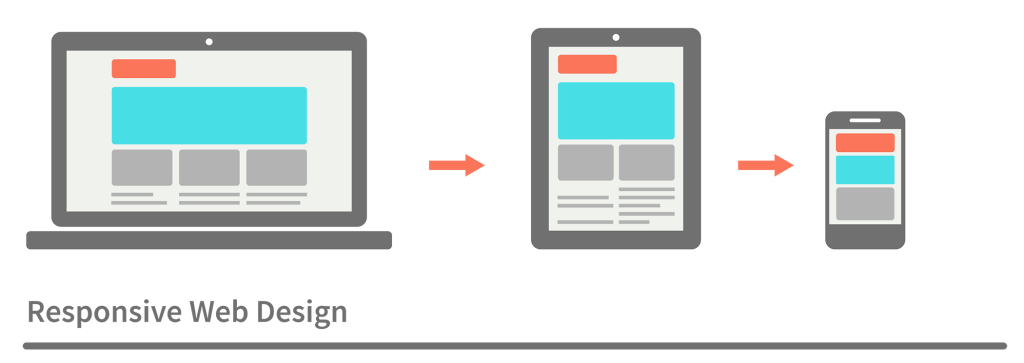
\includegraphics[width=1.0\textwidth]{figures/responsiveDesign}
    \caption{Ukázka responzivního designu mezi zařízeními. \cite{responsive_design}}
    \label{fig:responsive-design-example}
\end{figure}

\section{Analýza populárních deskových her}
\label{sec:popular-board-games-analysis}
Deskových her je v dnešní době na trhu velké množství, kde každým rokem se snaží noví nebo i stálí autoři proniknout ven s novými nápady nebo koncepty. Deskové hry lze tak rozdělit na několik herních žánru, jako jsou například hry strategické, kooperativní, party, rodinné nebo třeba karetní. Velká většina z těchto her se zaměřuje na její plný průběh na půdě hracího stolu, existují zde ale i hry, které do tohoto průběhu zapojují i externí zařízení, jako jsou speciální zařízení, mobilní telefony nebo laptopy. Tyhle hry se nazývají hry hybridní, kde jejich bližší definici popíšu v následující sekci.

\subsection*{Hybridní hry}
\label{subsec:popular-board-games-analysis-hybrid-games}
Jak již bylo zmíněno o sekci výše, hybridní hry jsou hry takové, které kombinují jednotlivé funkční prvky z her fyzických nebo digitálních. Jednoduše se tak dá řici, že hybridní hra je hra taková, které má jakékoliv napojení na technologii. Mezi hry hybridní tak patří například populární hra \textit{Monopoly}, která použivá speciální bankovní zařízení používané pro správu financí nebo hra \textit{XCOM: The Board Game}, která využívá mobilní aplikaci pro správu herního průběhu.

\subsection{Populární deskové hry}
\label{subsec:popular-board-games-analysis-popular-games}
Populárních deskových her je na světě velké množství, pro tuto analýzu jsem si vybral několik her, které mi jsou nejbližší a již jsem měl možnost si je zahrát. Díky této zkušenosti můžu lépe popsat možnosti a prvky, které tyto hry obsahují. Mezi tyto stolní hry patří například \textit{Carcassonne}, \textit{Bang!}, \textit{Codenames} nebo \textit{Gloomhaven}.

\subsubsection{Carcassonne}
\label{subsubsec:popular-board-games-analysis-carcassonne}
\textcolor{red}{DOPLNIT -- Popsat hru jak funguje, cíl, jaké prvky obsahuje, rozšíření. Poté její online verze.}

\subsubsection{Bang!}
\label{subsubsec:popular-board-games-analysis-bang}
\textcolor{red}{DOPLNIT -- Popsat hru jak funguje, cíl, jaké prvky obsahuje, rozšíření. Poté její online verze.}

\subsubsection{Codenames (Krycí jména)}
\label{subsubsec:popular-board-games-analysis-codenames}
\textcolor{red}{DOPLNIT -- Popsat hru jak funguje, cíl, jaké prvky obsahuje, rozšíření. Poté její online verze.}

\subsubsection{Gloomhaven}
\label{subsubsec:popular-board-games-analysis-gloomhaven}
\textcolor{red}{DOPLNIT -- Popsat hru jak funguje, cíl, jaké prvky obsahuje, rozšíření. Poté její online verze.}

\section{Administrativní prvky}
\label{sec:admin-elements}
Každé administrativní rozhraní se skládá z několika základních prvků, které umožňuje uživatelům s administrativními oprávněním provádět specifické úkony nebo měnit kompletní nastavení aplikace. Mezi takové prvky patří například správa uživatelů, obsahu, nastavení, zobrazení statistik nebo přehled logů. V následujících podkapitolách se blíže zaměřím na tyto jednotlivé prvky.

\subsection{Správa uživatelů}
\label{subsec:admin-elements-user-management}
Správa uživatelů je nedílnou součástí každého sofistikovaného systému nebo aplikace, která umožňuje administrátorům ovlivňovat kdo může přistupovat a jednotlivým částem systému. Tento prvek systému tak umožňuje nejen přidávat, odstraňovat nebo měnit uživatele, ale také udělovat jejich oprávnění, role nebo měnit nastavení. Mezi časté role patří například \textit{administrátor}, \textit{editor}, \textit{moderátor} nebo výchozí \textit{uživatel}. Každá role má přidělený seznam oprávnění, které určují co může uživatel dělat a co ne.

Tento přístup tak umožňuje vytvářet hierarchii uživatelů, kde administrátor má plný přístup ke všem funkcím aplikace, zatímco uživatel má pouze omezený přístup, čímž tak zvyšuje bezpečnost a efektivitu aplikace. Správa uživatelů také často obsahuje nástroje pro sledování aktivity uživatelů nebo jejich audit.

\begin{figure}[H]
    \centering
    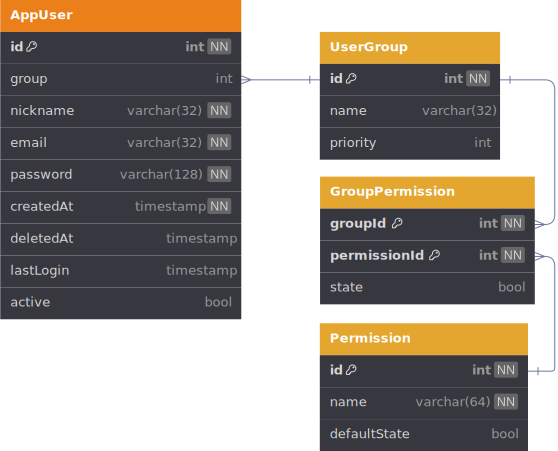
\includegraphics[width=0.7\textwidth]{diagrams/userManagement}
    \caption{Ukázka uložení uživatele v databázi. \cite{responsive_design}}
    \label{fig:user-management}
\end{figure}

\subsection{Správa obsahu}
\label{subsec:admin-elements-content-management}
Jako u správy uživatelů, správa obsahu z anglického jazyka \textit{\textquote{Content Management}} je dalším a hlavním pilířem administrativních rozhraní. Tento prvek tak umožňuje výše zmíněným rolím vytvářet, upravovat a odstraňovat obsah tak, že není nutné jakkoliv zasahovat do kódu aplikace nebo měnit čisté data ručně v databázi. Tento prvek je zásadní pro dynamické webové stránky, e-commerce platformy, blogy a další aplikace, které pravidelně mění svůj obsah nebo provádí jejich další vývoj.

Editace obsahu v aplikacích se provádí pomocí interaktivních editorů, které jsou součástí formulářů. Takové editory se nazývají WYSIWYG z anglického \textit{\textquote{What You See Is What You Get}}, tyto editory tak umožňují uživatelům editovat obsah aniž by museli znát HTML nebo CSS. Tento způsob editace je velmi oblíbený pro svou jednoduchost a přehlednost, která umožňuje i méně zkušeným uživatelům editovat obsah bez jakýchkoliv problémů. Mezi tyto populární editory patří CKEditor\footnote[1]{\url{https://ckeditor.com/}}, TinyMC\footnote[2]{\url{https://www.tiny.cloud/}} nebo Quill\footnote[3]{\url{https://quilljs.com/}}.

\subsection{Nastavení}
\label{subsec:admin-elements-settings}
Sekce pro nastavení se nachází v každém administrativním rozhraní a umožňuje tak administrátorům přizpůsobovat aplikaci podle specifických potřeb a preferencí. To může zahrnovat širokou škálu možností začínající od změny barvy, jazyka, loga, až po pokročilé možnosti jako je změna způsobu zabezpečení, různé integrace třetích stran a časté upravování SEO nastavení, které zlepšuje viditelnost aplikace ve vyhledávačích.

\subsection{Statistiky}
\label{subsec:admin-elements-statistics}
Statistiky poskytují ucelený přehled o využití a výkonost aplikace. Kde se zaměřuje na analýzu návštěvnosti, sledování chování uživatelů nebo sledování výkonu aplikace. Tento prvek tak umožňuje administrátorům sledovat aktuální stav aplikace a provádět potřebné úpravy pro zlepšení výkonu nebo zvýšení návštěvnosti.
Tyto statistiky se většinou zobrazují v podobě grafů, tabulek nebo zpráv, které poskytují uživatelům přehledné informace o aktuálním stavu aplikace.

Jako často používané nástroje pro sledování statistik se používají Google Analytics\footnote[4]{\url{https://analytics.google.com/}}, Matomo\footnote[5]{\url{https://matomo.org/}} nebo Yandex Metrica\footnote[6]{\url{https://metrica.yandex.com/}}. Při používání těchto nástrojů třetích stran je tak nutné dbát na zabezpečení a ochranu uživatelských dat, které tyto nástroje zpracovávají.

\subsection{Logování}
\label{subsec:admin-elements-logs}
Systém logování je nezbytným nástrojem pro monitorování a diagnostiku problému v aplikaci. Umožňuje tak zaznaménávat události jako jsou chyby, varování, informační zprávy nebo auditní záznamy o aktivitách uživatelů. Zpětné zobrazování těch záznamu tak pomáhá uživatelům rychle identifikovat a vyřešit problém čímž zajišťují bezpečný a nepřetržitý průběh aplikace.

\section{Administrativní značky}
\label{sec:admin-tags}
Administrativními značkami se rozumí prvky HTML, které jsou specifické pro přijímání požadavků od uživatele nebo uživateli předávají informace. Mezi takové značky patří například formuláře, tlačítka, tabulky nebo grafy. Jednotlivé značky se v nižších podkapitolách pokusím blíže přiblížit.

\subsection{Menu}
\label{subsec:admin-tags-menu}
Menu je zásadním navigačním prvkem v jakémkoliv rozhraní, umožňující uživatelů snadný přístup k rozdílným částem aplikace. Tento prvek se tak často nachází v horní částí aplikace nebo v její levé části a obsahuje tak odkazy na podřadné stránky. Důležitá je efektivnost navržení menu, kde se klade důraz na uživatelskou přívětivost a rychlou orientaci. Při velkém a rozsáhlém stromu menu tak v opačném případě dochází k častému zmatení uživatele, který pak často stránku opouští.

\subsection{Formulář}
\label{subsec:admin-tags-form}
Formuláře jsou klíčové pro interakci s uživatelem, neboť umožňují aplikaci přijímat datový vstup od uživatelů. Častým výskytem formulářů v administrativních rozhraních jsou stránky určené pro přihlášení, registraci, zadávání nebo úpravu dat. Formuláře se tak skládají z prvků jako jsou textová pole, výběrové seznamy, zaškrtávací políčka nebo obyčejné tlačítka pro provádění akce. U každého formuláře je tak důležité zabezpečení vstupu proti různým útokům, které dále budou popsány v sekci~\ref{sec:security}.

\subsection{Tlačítko}
\label{subsec:admin-tags-button}
Tlačítka jsou základním interaktivním prvkem, který umožňuje uživatelům provádět předem definované akce jako je například odeslání formuláře, potvrzení akce nebo přechod na jinou stránku. V ideálním případě by tak všechna tlačítka měla být navržena tak, aby byla pro uživatele snadno rozpoznatelná a měla tak jasně definovanou funkci. Tlačítka se tak často využívají v kombinaci s formuláři, tabulkami nebo odkazy v menu.

\subsection{Tabulka}
\label{subsec:admin-tags-table}
Tabulky jsou nezbytné pro zobrazení a přehlednou organizaci dat v strukturované formě. V administrativních rozhraních se tak tabulky využívají k zobrazení malého i velkého množství dat, například tak k zobrazení seznamu uživatelů, záznamu nebo třeba i statistikám. K tabulkám se pak vážou i často využívané prvky jako je možnost řazení, filtrování a stránkování záznamu což je nezbytné k správě velkého množství dat.

\subsection{Graf}
\label{subsec:admin-tags-chart}
Grafy nebo diagramy jsou významným prvkem pro vizualizaci dat, která se vyskytují většinou u komerčních administrativních rozhraní více než u rozhraní, které se čistě zaměřují na správu obsahu. Tyto grafy nám tak pomáhají lépe pochopit vztahy mezi data a čistě tak rozlišit vzory nebo trendy. Grafy se tak využívají pro zobrazení statistik, vývoje, analytiky a dalších měřitelných dat.

\subsection{Modální okno}
\label{subsec:admin-tags-modal}
Modální okna jsou interaktivní dialogové okna, které přitahují pozornost uživatele tak aby vykonal určitý úkon před tím, než bude moci pokračovat dále v předchozím úkonu. Tyto okna se tak často využívají pro potvrzení akce, zobrazení upozornění nebo detailního zobrazení obsahu. Jejich správné využití tak mnohem zlepšuje uživatelskou přívětivost tím, že umožní uživateli rychle reagovat bez nutnosti opustit aktuální kontext úkonu.

\section{Zabezpečení}
\label{sec:security}
Zabezpečení v rozhraních je dalším z mnoha důležitých aspektu neli ten nejdůležitější neboť se zde setkáváme s citlivými daty, které by při odcizení mohlo mít nemalý dopad na uživatele nebo samotnou aplikace. Zabezpečení se tak dělí na několik oblastí, kde každý z nich má své specifické praktiky a techniky, které zvyšují bezpečnost aplikace. V dnešní době existuje mnoho způsobu, jakým lze na danou aplikaci nebo uživatele útočit, mezi jedny z nejčastější patří \textit{SQL Injection}, \textit{Cross-Site Scripting} nebo \textit{Cross-Site Request Forgery}. V následujících podkapitolách se tak zaměřím na tyto jednotlivé oblasti.

\subsection{Autentizace}
\label{subsec:security-authentication}
Autentizace je proces, kde dochází k ověřování identity uživatele při vstupu do systému. Jedná se tak o první krok, který systém provádí před tím, než uživatel může dále interagovat s aplikací. Autentizace se tak dělí na několik základních metod, jako je přístup s \textit{uživatelským jménem a heslem}, \textit{tokenem}, \textit{biometrickými údaji} nebo \textit{certifikáty}. Každá z těchto metod má své výhody a nevýhody, které se tak většinou volí dle potřeb aplikace nebo uživatele.

Jako druhy ošetření autentizace se využívá praktik:
\begin{itemize}
    \item \textbf{Silná hesla} -- Uživatel je donucen používat heslo, které spadá do nastavené politiky administrátorem systému. Nejčastěji tak hesla musí kombinovat velká a malá písmena, čísla a speciální znaky, kde celkově heslo musí dosahovat minimálně délky 8 znaků.
    \item \textbf{Dvoufaktorová autentizace} -- Jedná se druhou vrstvu zabezpečení, kde po obyčejném přihlášení uživatele do systému, je vyžadován druhý faktor ověření. Tento faktor může být například SMS zpráva, e-mail nebo digitální token, který uživatel musí zadat pro dokončení přihlášení.
    \item \textbf{Omezení počtu pokusů} -- Tato prevence se zaměřuje na takzvaný útok hrubou sílou z anglického jazyka \textit{\textquote{Brute Force}}, kde se útočník pokouší proniknou za pomocí slovníku hesel, ale je zablokován po několika neúspěšných pokusech.
\end{itemize}

\subsection{Autorizace}
\label{subsec:security-authorization}
Autorizace se zaměřuje na rozřazení uživatelů do skupin nebo rolí, kde ověřují, zda uživatel má oprávnění provádět danou akci v systému. Nejlepším princem je tak tzv. \textit{Princip nejmenších oprávnění}, který říká, že uživatel by měl mít pouze ta oprávnění, která potřebuje pro vykonání své práce a nic víc. Často tak oprávněni uživatelé dostávají vyšší oprávnění pouze dočasně po dobu své práce a poté jsou oprávnění zpět odebrány.

\subsection{Šifrování}
\label{subsec:security-encryption}
Šifrování je procesem konverze dat do formátu, který není čitelný bez dešifrovacího klíče. Tento proces se tak často využívá u důležitých citlivých údajů jako jsou například adresy, hesla nebo platební údaje. Šifrování se tak dělí na několik základních metod, jako je \textit{symetrické šifrování}, \textit{asymetrické šifrování} nebo \textit{hashování}. Při výběru metody šifrování je tak důležité zvolit takovou metodu, která je dostatečně bezpečná a zároveň efektivní. Pro zachování zabezpečení komunikace se tak používá webový protokol HTTPS, který šifruje data za nás.

\subsection{Zabezpečení formulářů}
\label{subsec:security-forms}
Zabezpečení formulářů je klíčových prvkem pro ošetření vstupu dat od uživatele. Uživatel neboli útočník se v tomto případě pokouší o vložení škodlivého kódu do formuláře, který může mít za následek přeskočení přihlášovacích údaju, získání citlivých informací nebo zneužití aplikace. Pro ošetření formulářů se tak využívají techniky jako je \textit{validace}, \textit{filtraci} nebo \textit{escapování}.

\subsection{Zabezpečení proti útokům}
\label{subsec:security-attacks}
V moderních době počítačů existuje mnoho možnosti, jak útočnicí se mohou pokoušet proniknout do aplikace. Mezi nejčastější útoky patří \textit{SQL Injection}, \textit{Cross-Site Scripting}, \textit{Cross-Site Request Forgery} nebo \textit{Session Hijacking}. Tyto útoky se tak zaměřují na různé části aplikace, kde se snaží získat citlivé informace, zneužít aplikaci nebo získat kontrolu nad uživatelem. Pro ošetření je tak nutné implementovat několik zabezpečovacích vrstev, které tak eliminují riziko útoků.

\subsubsection*{SQL Injection}
\label{subsubsec:security-attacks-sql-injection}
SQL Injection je druh útoků, kde ůtočník vkládá neboli "injektuje" škodlivý SQL kód do vstupu formuláře, který je poté zpracováván databázovém systémem. Pokud nedojde k ošetření vstupu, útočník tak může docílit k neautorizovanému přístupu k databázi, získání citlivých informací nebo dokonce k úplnému smazání databáze.

\textbf{Obrana:} Použitím parametrizovaných dotazů, kde dochází k bezpečnému vložení dat uživatele do SQL kódu. Dále je možné omezit přístupová oprávnění uživatele databáze na minimum.

\subsubsection*{Cross-Site Scripting}
\label{subsubsec:security-attacks-cross-site-scripting}
Cross-Site scripting je dalším z druhů útoku, kde útočník podobně jako u \textit{SQL Injection} vkládá do formuláře škodlivý kód. Zde se zde ale nejedná o kód SQL ale o kód JavaScriptu. Tento kód tak může v pozadí nenápadně provádět akce, které můžou vést k odcizení cookies nebo session tokenů.

\textbf{Obrana:} Sanitace všech uživatelských vstupů. Úplné odebrání HTML značek z vstupních dat.

\subsubsection*{Cross-Site Request Forgery}
\label{subsubsec:security-attacks-cross-site-request-forgery}
Cross-Site Request Forgery je útok, pri kterém útočník využívá fakt, že daný uživatel je již autorizovaný na dané stránce. Uživatel tak po otevření odkazu je přesměrován na cílovou stránku, kde se provede nežádaná akce pod účtem uživatele.

\textbf{Obrana:} Implementace CSRF tokenu v formuláři, který zajišťuje, že požadavek přichází od správného uživatele.

\subsubsection*{Session hijacking}
\label{subsubsec:security-attacks-session-hijacking}
Session hijacking se váže na \textit{Cross-Site Scripting}, kde útočník již obdržel uživatelovu session a může tak provádět akce pod uživatelským účtem aniž by se musel sám přihlásit.

\textbf{Obrana:} Použití HTTPS protokolu, který šifruje data. Omezení platnosti session tokenů, použití dvoufaktorové autentizace a nastavení správných cookie atributů.
\newline

Každý z těchto výše zmíněných útoků představuje vážnou hrozbu pro bezpečnost aplikace a její uživatele. Proto je tak nutné dbát na správné zabezpečení aplikace a v pravidelných intervalech provádět bezpečností opatření, tak aby došlo k minimalizaci rizika útoků.

\endinput


\chapter{Závěr}
\label{ch:conclusion}

V této bakalářské práci jsme se zaměřili na návrh a implementaci administrativního rozhraní pro kompletní správu obsahu výpravně evoluční hry, která tak kombinuje prvky deskových a digitálních her. Cílem práce bylo vytvořit efektivní nástroj umožňující administrátorům správu herních prvků, jako jsou postavy, předměty, lokace, nepřátele a další. V průběhu práce byla provedena analýza existujících administrativních rozhraní zaměřená na jejich funkčnost a uživatelskou přívětivost, na základě které byla výsledná práce směřována.

Implementace administrativního rozhraní tak zahrnovala vytvoření funkčního prototypu, který umožňuje provádět operace nad objekty, jako je vytváření, editace, mazání nebo zobrazení detailů. Prototyp tak byl vyvíjen s obezřetnosti na možnost budoucího rozšíření a modulárnosti. Díky kombinaci moderních technologií bylo možné vytvořit uživatelsky přívětivé rozhraní s intuitivní navigací a bezpečnostními opatřeními.

Součástí této práce se tak dá považovat i spolupráce s ostatními členy týmu na vývoji herního designu, implementaci API nebo tvoření celkového obsahu hry, který lze vidět v zdrojových kódech přílohy \textit{TTS-Database}.

Kromě technické implementace byla také vytvořena uživatelská příručka, které je samostatně integrovaná do administrativního rozhraní. Uživatelskou příručku tak lze naleznout v kterékoliv sekci webu pod tlačítkem \textit{Help}. Tento manuál tak poskytuje dostatečné informace, které uživatelům umožňují efektivně využívat všechny funkce rozhraní.

Celkově tak lze konstatovat, že výsledný prototyp splňuje veškeré stanovené cíle dle zadání a představuje tak schopný nástroj pro správu obsahu hry. Díky možnostem rozšíření tak není v budoucnu problém rozhraní rozšířit o další aktualizace. Budoucí práce by tak mohla zahrnovat rozšíření o další nástroje jako je například statistika, záznam provedených akcí nebo celkově rozšířit možnost efektivněji spravovat obsah.

Ukázka výsledného rozhraní je možné vidět v příloze~\ref{ch:appendix-interface-screenshots}

\endinput

% Seznam literatury
\printbibliography[title={Literatura}, heading=bibintoc]

\end{document}
